\section{Short-Range Correlations\label{sec:srcs}}
%\subsection{Inclusive Measurements}
Short-range correlations offer access to understanding a more detailed picture of the high-momentum structure of nuclei as well as possible unique insight into the generation of the EMC effect.  Results from JLab's 6~GeV era have led to an investiation of a possible connection between the EMC effect and short-range NN behavior.  Inclusive experiments aim to measure precision cross section ratios at $x >$ 1, a region forbidden to the free nucleon.  Exclusive measurements yield a more detailed picture of the high momentum structure of nuclei and its isospin structure an many-body correlations.

For the inclusive case, the electron scattering probes high-momentum nucleons, typically defined as ones with momenta $\ge$300~MeV/c, typically a few tens of~MeV greater than the Fermi momentum for a given nucleus for $A>12$.  If the presence of these high-momentum nucleons is the result of SRCs, then the cross sections for A$>$2 will be re-scaled versions of the deuteron cross sections, signaling more SRCs and therefore more high-momentum nucleons in larger nuclei.   The observation of a plateau at $x>$1 in the $A/D$ cross-section ratios supports this picture.    Experimentally, the onset of the scaling plateau is observed at lower $x$ values as Q$^2$ increased, with the minimum $Q^2$ value taken to be about 1.4~GeV$^2$ illustrated with data from Ref.~\cite{Egiyan:2003vg}.  Cross section plateaus at $x>1$ were observed in several JLab experiments~\cite{Egiyan:2003vg, Fomin:2011ng} and is proportional to the relative number of high-momentum nucleons in $A$ with respect $D$, including the number of SRC pairs and higher order correlations.   %The pairs in a $A>2$ nucleus will experience center-of-mass motion due to the fields of the other nucleons and will redistribute some strength from the quasielastic peak to the tail of the momentum distribution, resulting in an enhancement in $A>2$ cross sections in the region of interest.  
%A convention of $a_2=\sigma_A/\sigma_D$ is used for raw cross section ratios and $R_{2N}$ for those corrected for the center-of-mass motion of the 2N pair. 

%The precision results from JLab E02-019~\cite{Fomin:2011ng} were used to study the nuclear dependence of SRCs. No simple dependence with $A$, density, separation energy or numerous other quantities~\cite{PhysRevC.86.065204} was observed.  However, a deviation of $^9$Be from a simple density dependence analogous to that of the EMC effect was noted.  This led to a number of correlation studies between the two different phenomena and a search for a potential causal effect~\cite{PhysRevC.86.065204, Hen:2012fm, Weinstein:2010rt}. % This is further discussed in Sec.~\ref{sec:SRC_EMC}.

There is an expectation to observe a second plateau at higher $x$ in $A/^3\mathrm{He}$ cross section ratios, corresponding to a relative number of 3N configurations in $A$ relative to $^3$He.  Several experiments ~\cite{PhysRevLett.96.082501, Fomin:2011ng, PhysRevC.97.065204} measured cross sections in the $x>2$ region, but none observed a plateau.  These measurements were performed for a range of $Q^2$ values in order to potentially map out the onset of a 3N plateau, analogously to the case of 2N SRC.  However, defining a kinematic threshold for 3N dominance is more difficult as there is more than a single configuration that the 3N correlation can take and there are additional dynamics to consider.  More detailed kinematic calculations have suggested that to see a second plateau over a meaningful $x$ range requires data at higher $Q^2$ values than any of the experiments have previously obtained~\cite{Fomin:2017ydn}.  Collecting adequate statistics for such a result on $^3$He is time prohibitive, and future experiments will more than likely look for the 3N plateau in $A/^4\mathrm{He}$ ratios.  This is expected as the cross section for $A=2$~or$3$ approaches zero for $x>2$ more quickly as well as distortion from center-of-mass motion for higher $A$. 

%\subsection{Exclusive Measurements}
%A program of exclusive measurements also yielded interesting results. A series of experiments to measure 2N knockout in a kinematic region of large $P_\mathrm{miss}$ that would correspond to a 2N SRC pair revealed that these pairs are predominantly $np$~\cite{Subedi:2008zz, Shneor:2007tu}.  This observation was consistent with the theoretical calculation~\cite{Schiavilla:2006xx} showing a tensor force dominance in the regime where the first measurements were done and also predicted a weakening of $np$ dominance with growing $P_\mathrm{miss}$, which follow-up measurements appear to support~\cite{Korover:2014dma}, although with uncertainties that prevent conclusive statements. 


%\subsection{SRC Summary}
%Going into the 12~GeV era at JLab, our future measurements are informed by the following lessons from previous experiments
%\begin{itemize}
%\item Scaling of $A/D$ cross section ratios at $x>$1 observed
%\item No clear nuclear dependence of the $a_2$ ratios
%\item $NP$ dominance of SRC pairs (while significant contributions from FSI are present, they are unlikely to mimic the physics result)
%\item No 3N SRC plateau observed
%\end{itemize}

%\subsection{\label{sec:SRC_EMC}SRC- EMC connection}
%When neither SRCs or EMC effect showed a simple nuclear dependence, but both exhibited the same nuclear outliers, several analyses were done to examine the correlation between the two physical phenomena~\cite{PhysRevC.86.065204, Hen:2012fm, Weinstein:2010rt}.  On the surface, it might very well be a coincidence: SRCs are a measure of quasielastic cross sections, whereas the EMC effect probes DIS quark distributions.  Yet, there is room for the two to be related, as the cause for the nuclear modification of structure functions is not understood, and it could come from short-range dynamics probed by SRC measurements.   The other possibility is that both effects arise as the result of the same underlying mechanism rather than having a causal relationship.  Multiple corrections to SRC and EMC measurements were applied to check the robustness of the correlation, but at the end of the, the existing measurements are not precise enough nor span enough nuclei for any meaningful conclusions to be drawn.
%
%  Recent work in % FIXME Ref~\cite{} 
%proposes a new model for this that consists of a free structure function piece as well as a piece that depends on SRC, and it  reduces the EMC effect to a %dependence on the number of protons in the nucleus.  \textit{Wait...is that right}
%\begin{figure}[htb]
%  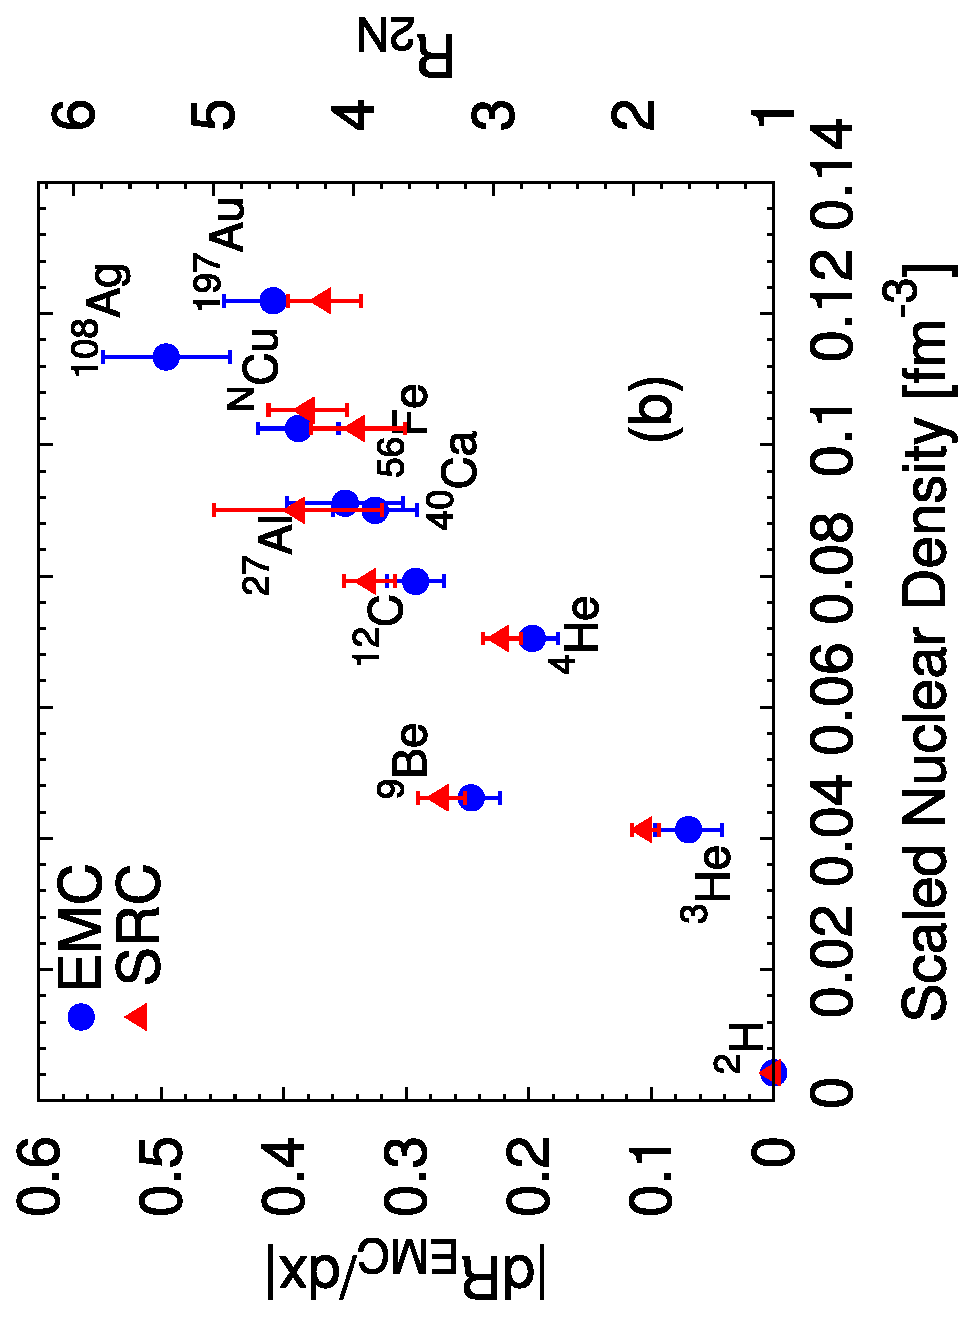
\includegraphics[angle=270, width=\columnwidth]{plots/emc_src_vs_scaled_dens_all.eps}
%  \caption{Size of the EMC effect (left axes) as well as the number of SRC pairs (right axes) as a function of scaled nuclear density}
%  \label{fig:src_emc}
%\end{figure}

%\subsection{Quarks at $x>$1}
%Quasielastic kinematics at $x>$1 probe moving nucleons, but if we increase the Q$^2$, the inelastic contribution begins to dominate, allowing us to access quark distributions. Existing JLab data have a limited range in $x$ and require the application of the of so-called "target-mass corrections" (TMCs) to extract the Q$^2\rightarrow\infty$ structure function limit.  This analysis was done for the E02-019 data, showing that the data are on the edge of... being useful?


